\documentclass[10pt,aspectratio=169
	%,handout
	]{beamer}
	\usetheme[
	%%% options passed to the outer theme
	%   rotationcw,          % change the rotation direction from counter-clockwise to clockwise
		sectionpages, 		% show section pages
		logo={_figures/logo-federico-II-blue.png}
	]{UniNA}
	%\graphicspath{ {./images} }
	%\setbeamercovered{transparent}
	
	\usepackage[utf8]{inputenc}
	\usepackage[italian]{babel}
	\usepackage[T1]{fontenc}
	\usepackage{tikz}
	\usepackage{multimedia}
	\usepackage{tabulary}

	\usepackage[scaled]{beramono}     %mono?
	\usepackage[scale=1.15]{AlegreyaSans}
	
	\title[Stabilizzazione nel piano di Gough-Stewart] %shown at the top of frames
	{\huge Stabilizzazione nel piano\\ di Gough-Stewart} %shown in title frame
	%\subtitle{M.Sc. Thesis in Computer Science}  % could also be a conference name
	
	%\date{December 6, 2018} %explicitly set date instead of \today
	
	\author[Daniele Facco]%shown at the top of frames
	{%shown in title frame
		{\footnotesize Presentato da}\\
		Daniele \textsc{Facco}%
	}
	
	% - Give the names in the same order as they appear in the paper.
	% - Use the \inst{?} command only if the authors have different
	%   affiliation. See the beamer manual for an example
	
	\institute[
		Dipartimento di ingegneria e architettura\\
		Università degli Studi di Trieste\\
		Italia
	]
	{% is placed on the bottom of the title page
		Università degli Studi di Trieste
	}

	\begin{document}

	\maketitle

	% TOC
	\begin{frame}{Argomenti trattati}{}
		\tableofcontents
	\end{frame}


	\section{Obiettivi del progetto}
	\begin{frame}{Obiettivi del progetto}
	\begin{enumerate}[<+->]
		\item Realizzare una piattaforma di Gough-Stewart con piano resistivo
		\item Implementare il controllore PID
		\item Stabilizzare la pallina su diversi punti piano
		\item Eseguire un controllo dinamico tracciando le figure di Lissajous
	\end{enumerate}

	\end{frame}


	\section{Introduzione}
	\subsection{Piattaforma di Gough-Stewart}
	% motivation for creating this theme
	\begin{frame}{Introduzione}{Piattaforma di Gough-Stewart}

	\begin{columns}
	\column{0.5\textwidth}
	%Stabilizzazione di una pallina su un piano mediante l'uso di una piattaforma di Gough-Stewart.
	
	\begin{itemize}
		\item Robot parallelo
		\item Esapode
		\item 6 gradi di libertà
		\item Largo impiego industriale
		\item Utilizzo attuatori rotativi
	\end{itemize}
	\column{0.5\textwidth}
	\centering 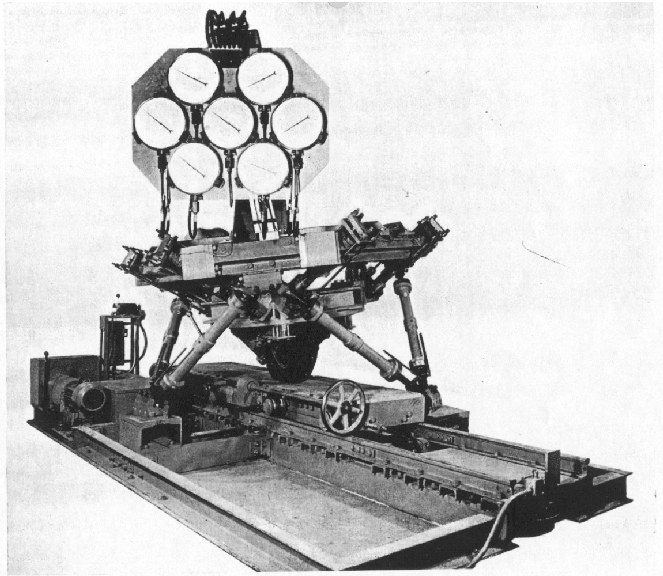
\includegraphics[width=\textwidth]{./images/gough.png}
	\end{columns}
		%\end{block}
	\end{frame}
	
	\subsection{Tecnologie impiegate}
	\begin{frame}{Introduzione}{Tecnologie impiegate}
		%\begin{block}{Why the UniNA beamer theme?}

	\begin{columns}
	\column{0.3\textwidth}
	%Stabilizzazione di una pallina su un piano mediante l'uso di una piattaforma di Gough-Stewart.
	
	\begin{itemize}
		\item Arduino
		\item Servomotori
		\item Piano resistivo
		\item Ponte ad H
	\end{itemize}
	\column{0.7\textwidth}
	\begin{tabular}{cc}
	\hspace{0.5cm}
  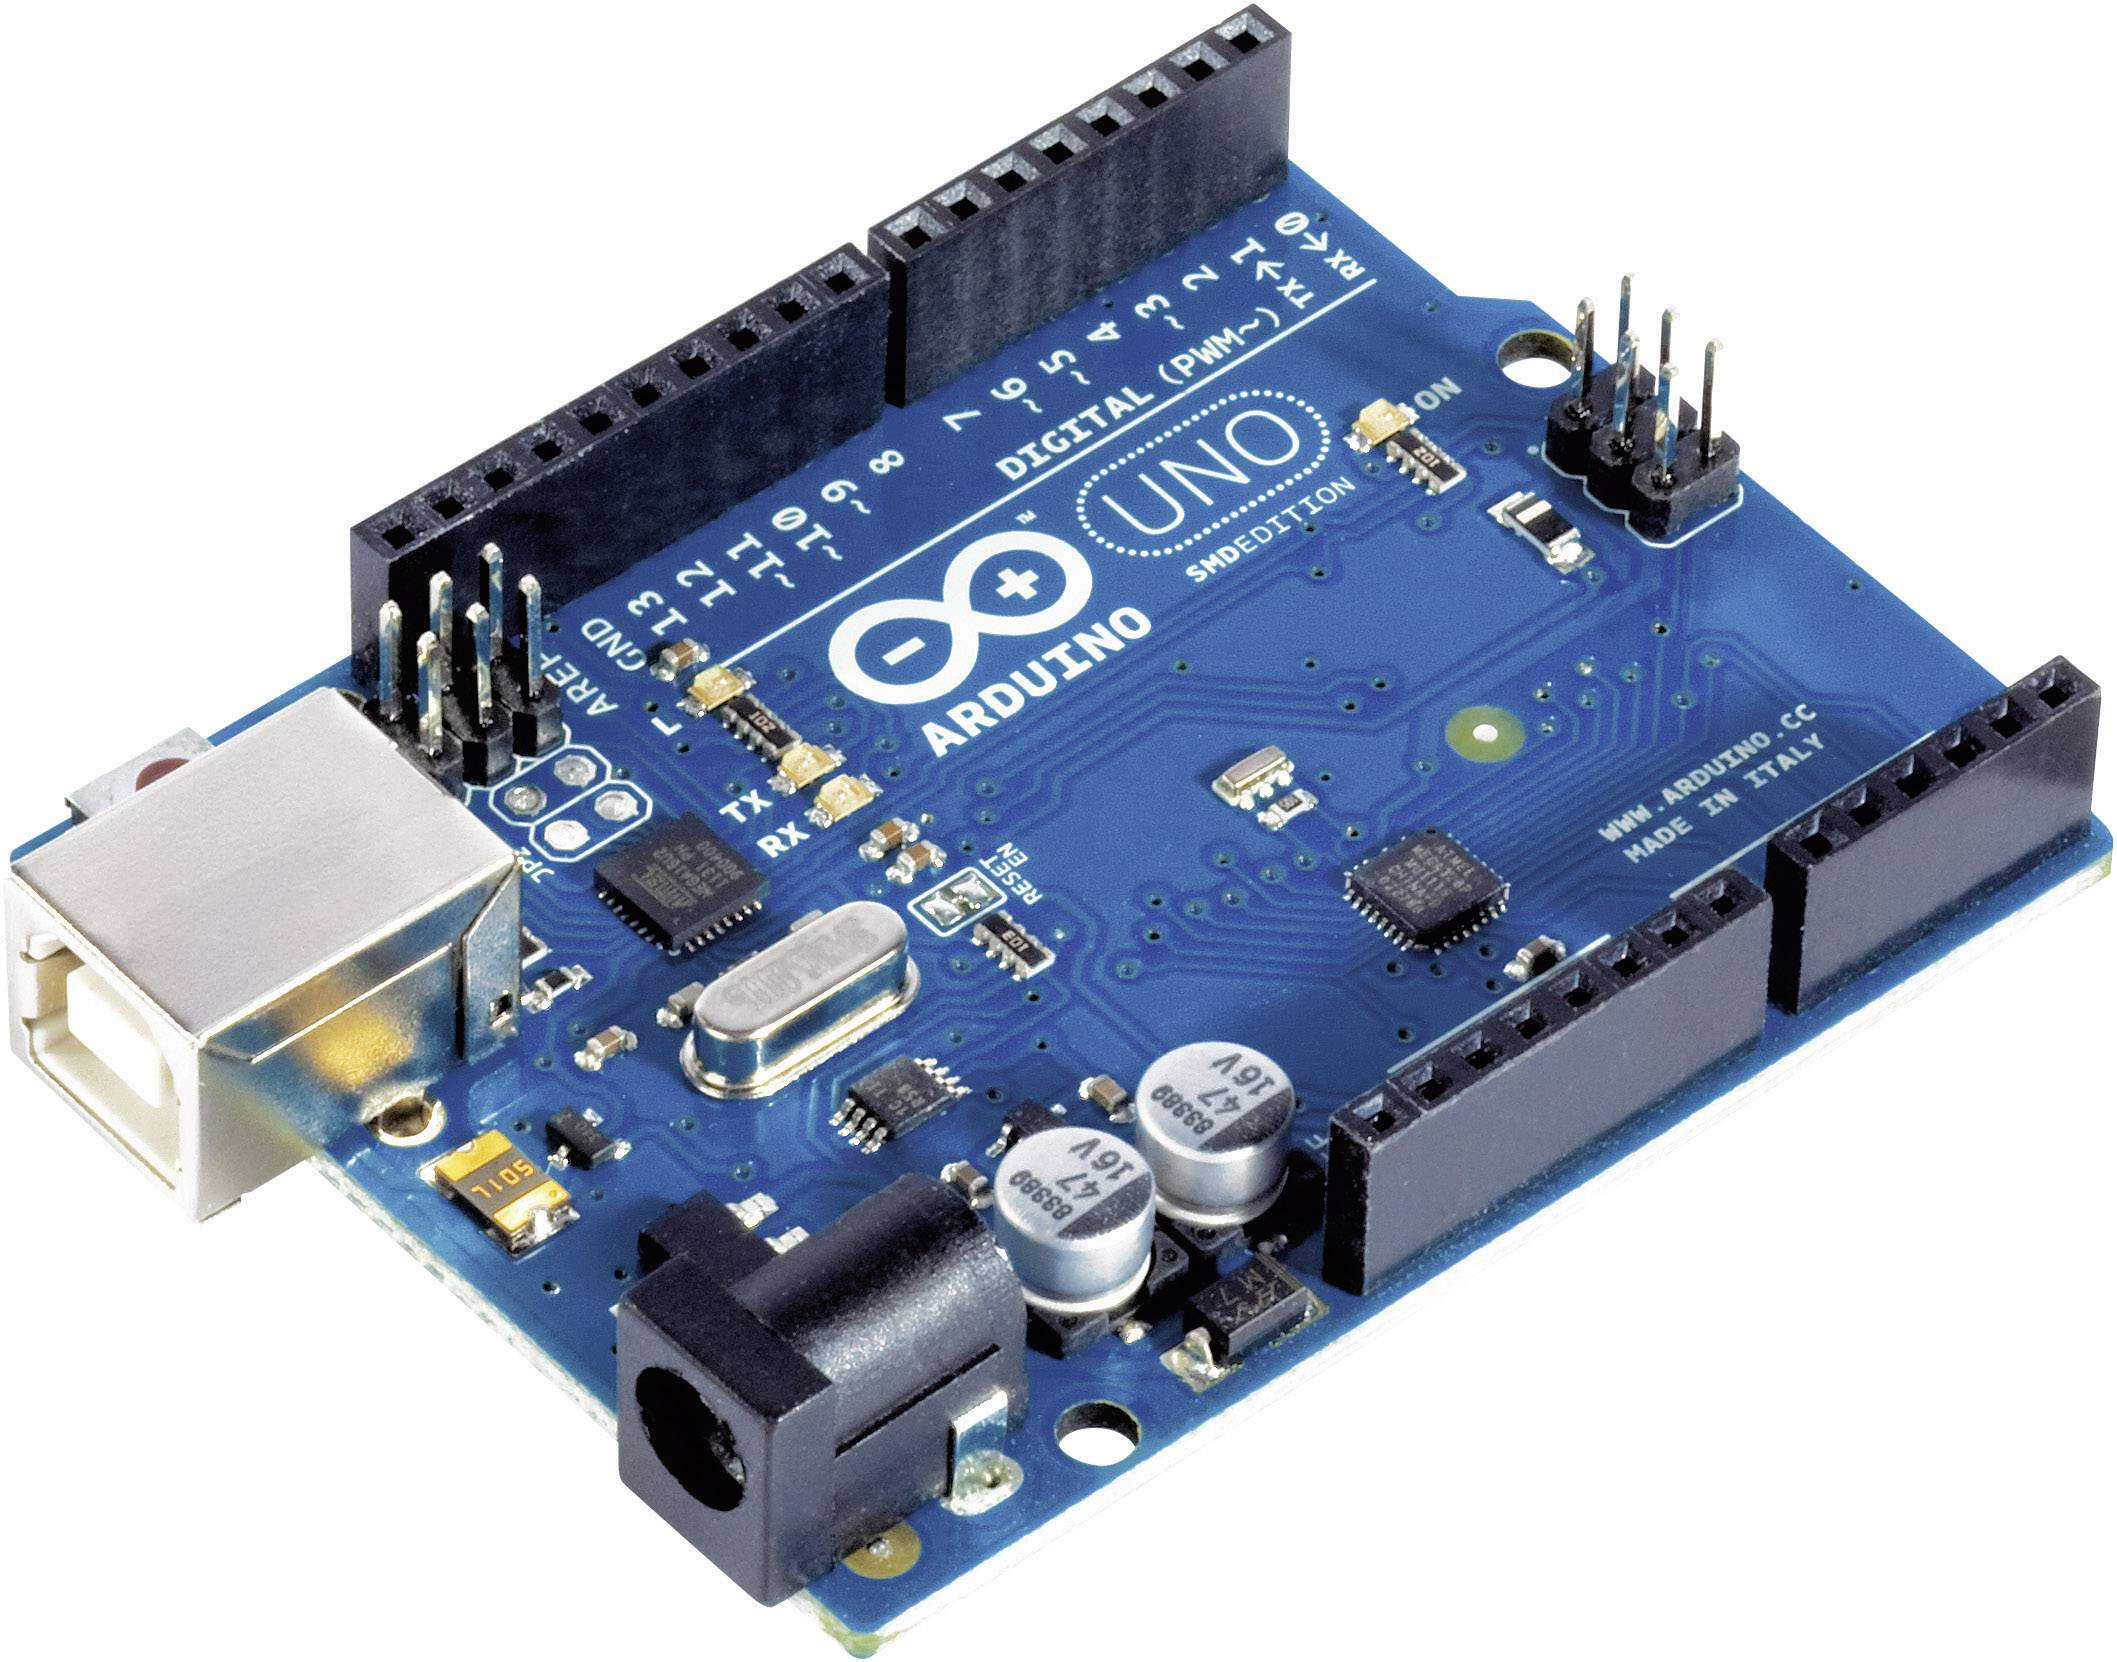
\includegraphics[height=0.3\textheight]{images/1.jpg}
  &
  \hspace{0.3cm}
  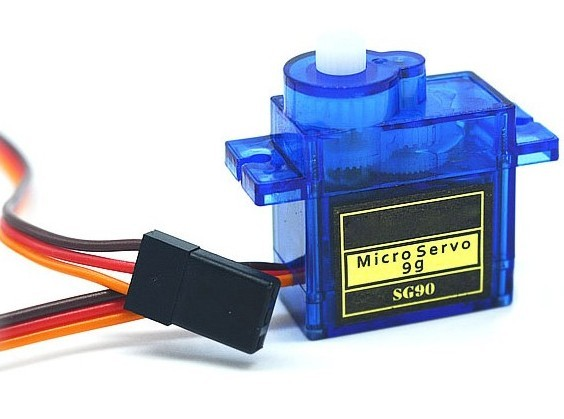
\includegraphics[height=0.3\textheight]{images/2.jpg}
 \end{tabular}

\begin{tabulary}{\linewidth}{CC}
  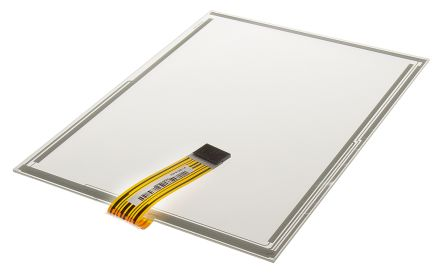
\includegraphics[height=0.3\textheight]{images/3.jpg}
  &
  \hspace{0cm}
  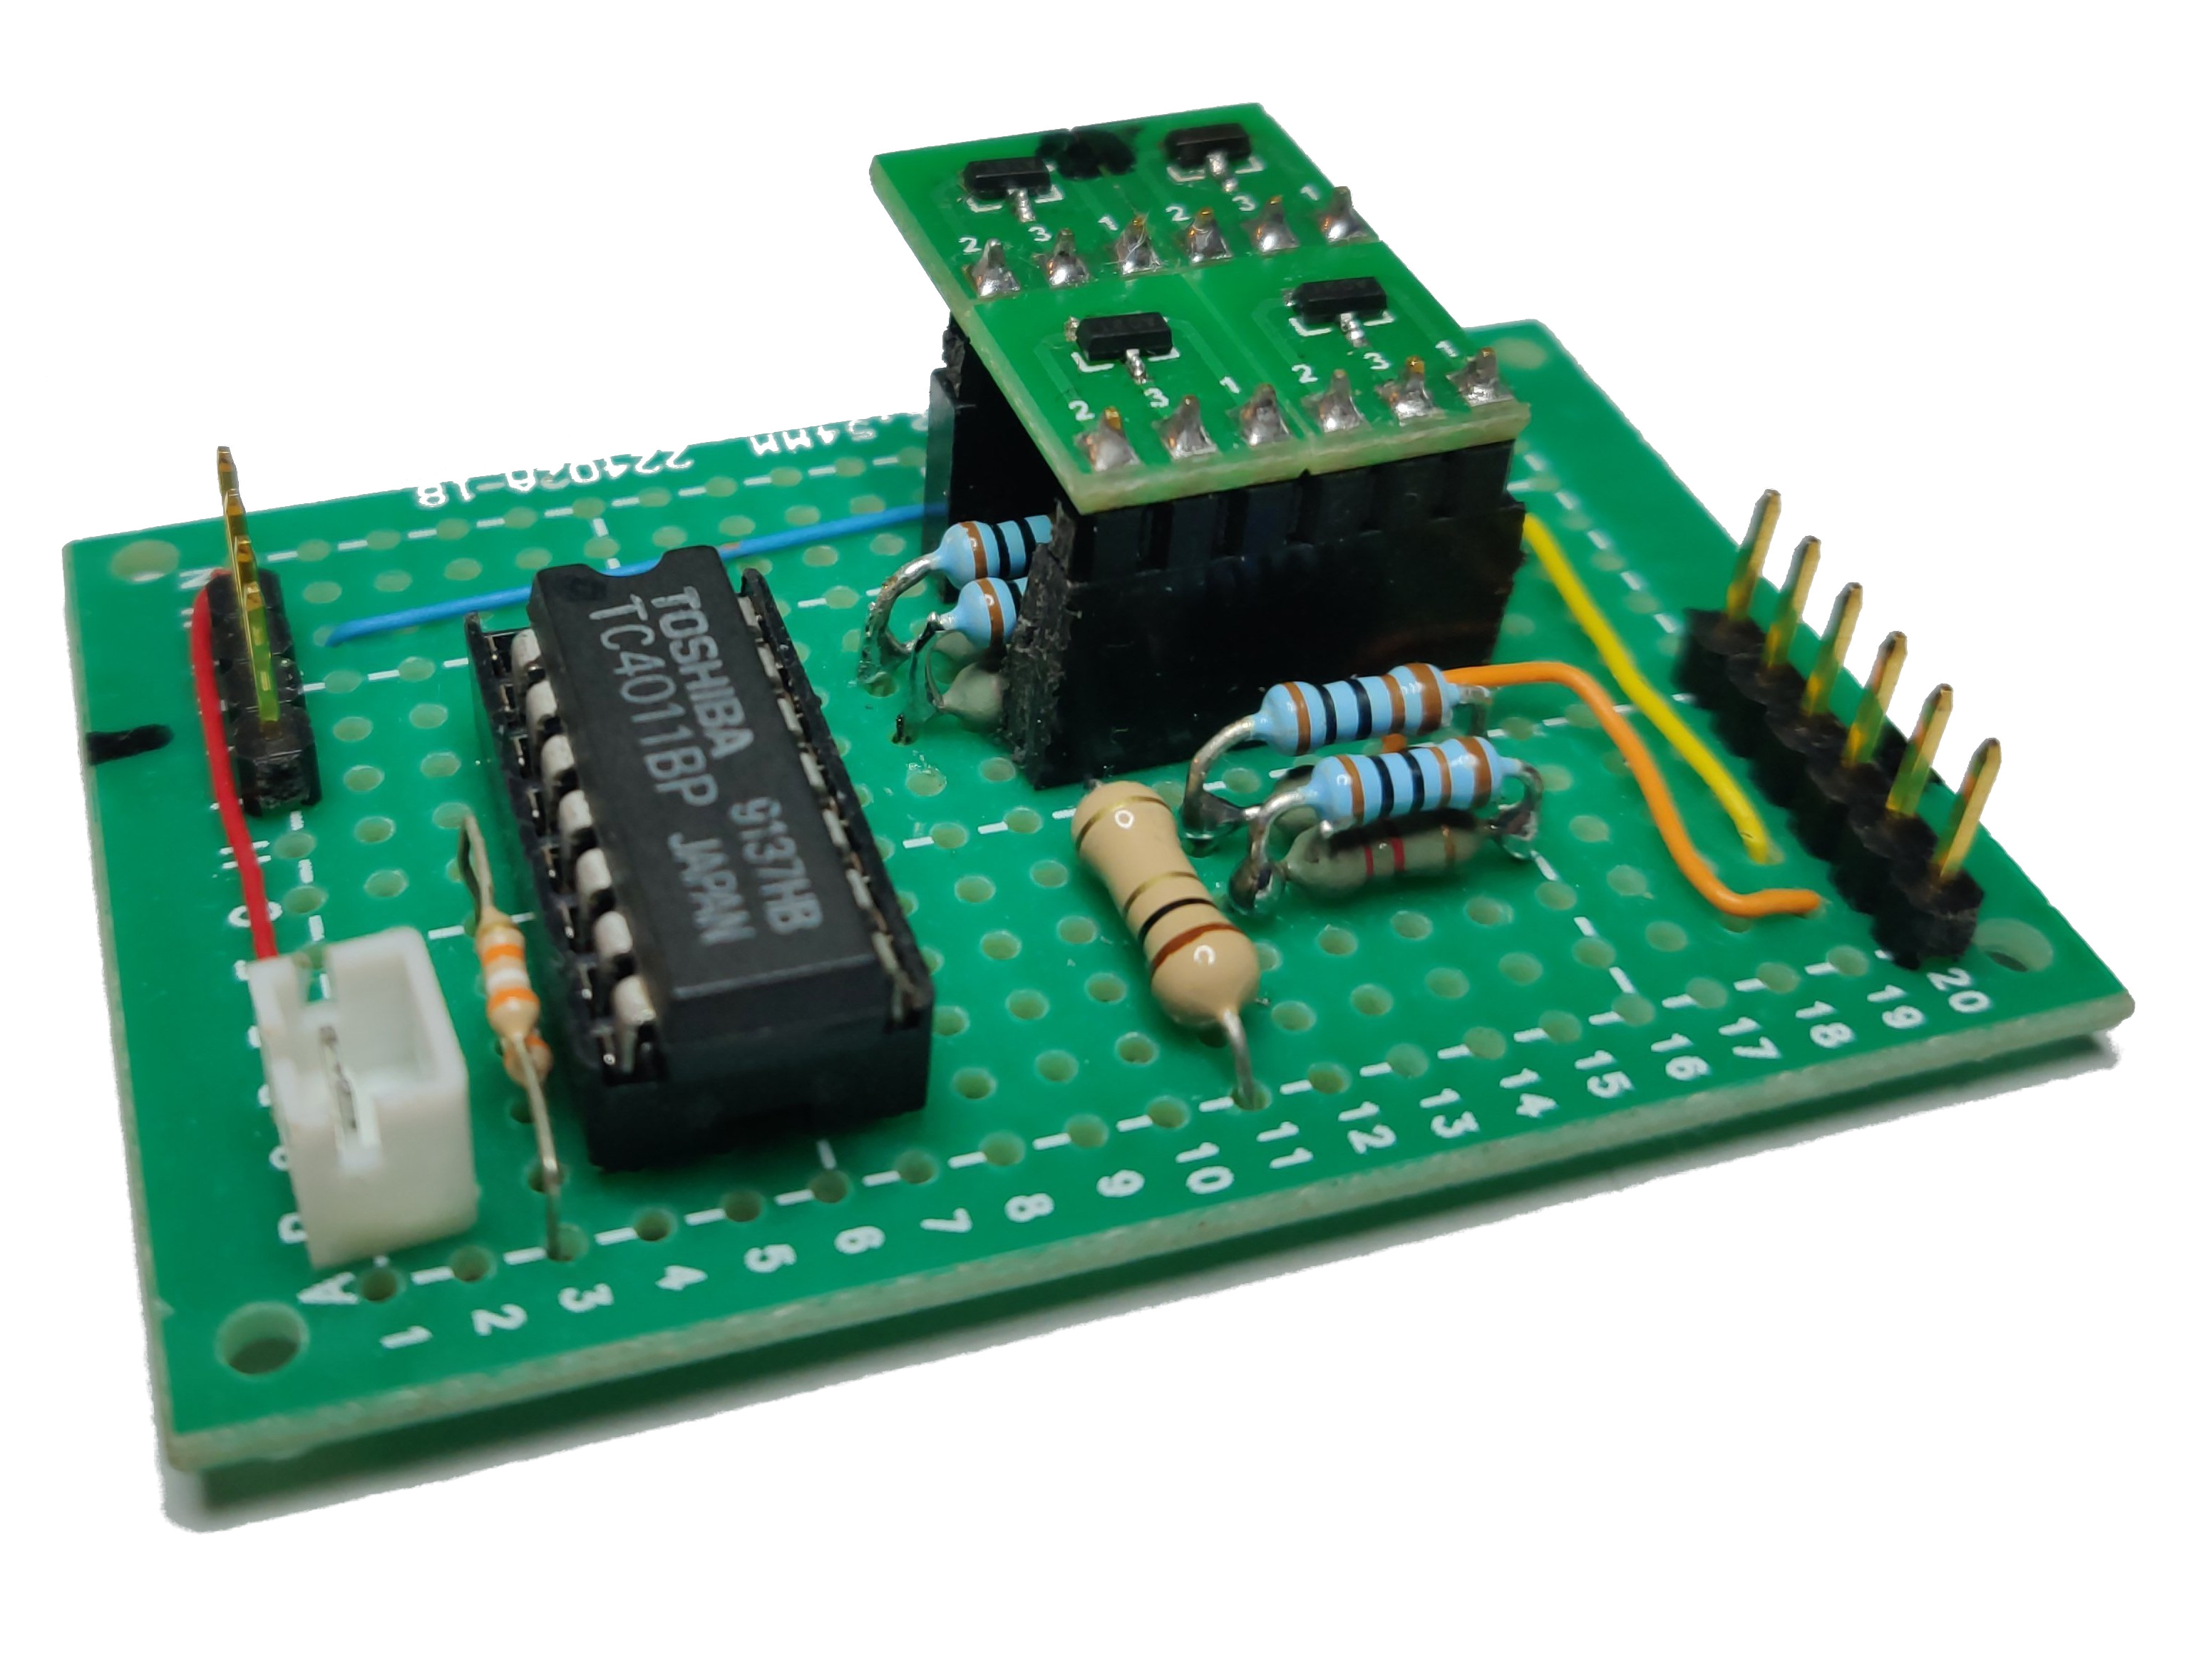
\includegraphics[height=0.3\textheight]{images/4.jpg}
 \end{tabulary}

	\end{columns}
		%\end{block}
	\end{frame}
	
	\begin{frame}{Introduzione}{Realizzazione ponte ad H}

	\begin{columns}
	\column{0.4\textwidth}
	%Stabilizzazione di una pallina su un piano mediante l'uso di una piattaforma di Gough-Stewart.
	
	\begin{itemize}
		\item Pilotare piano resistivo
		\item MOSFET
		\item Gradiente di tensione alternato sugli assi $x$ e $y$
		\item Misurare e limitare lo shoot-through
	\end{itemize}
	\column{0.6\textwidth}
	\centering
	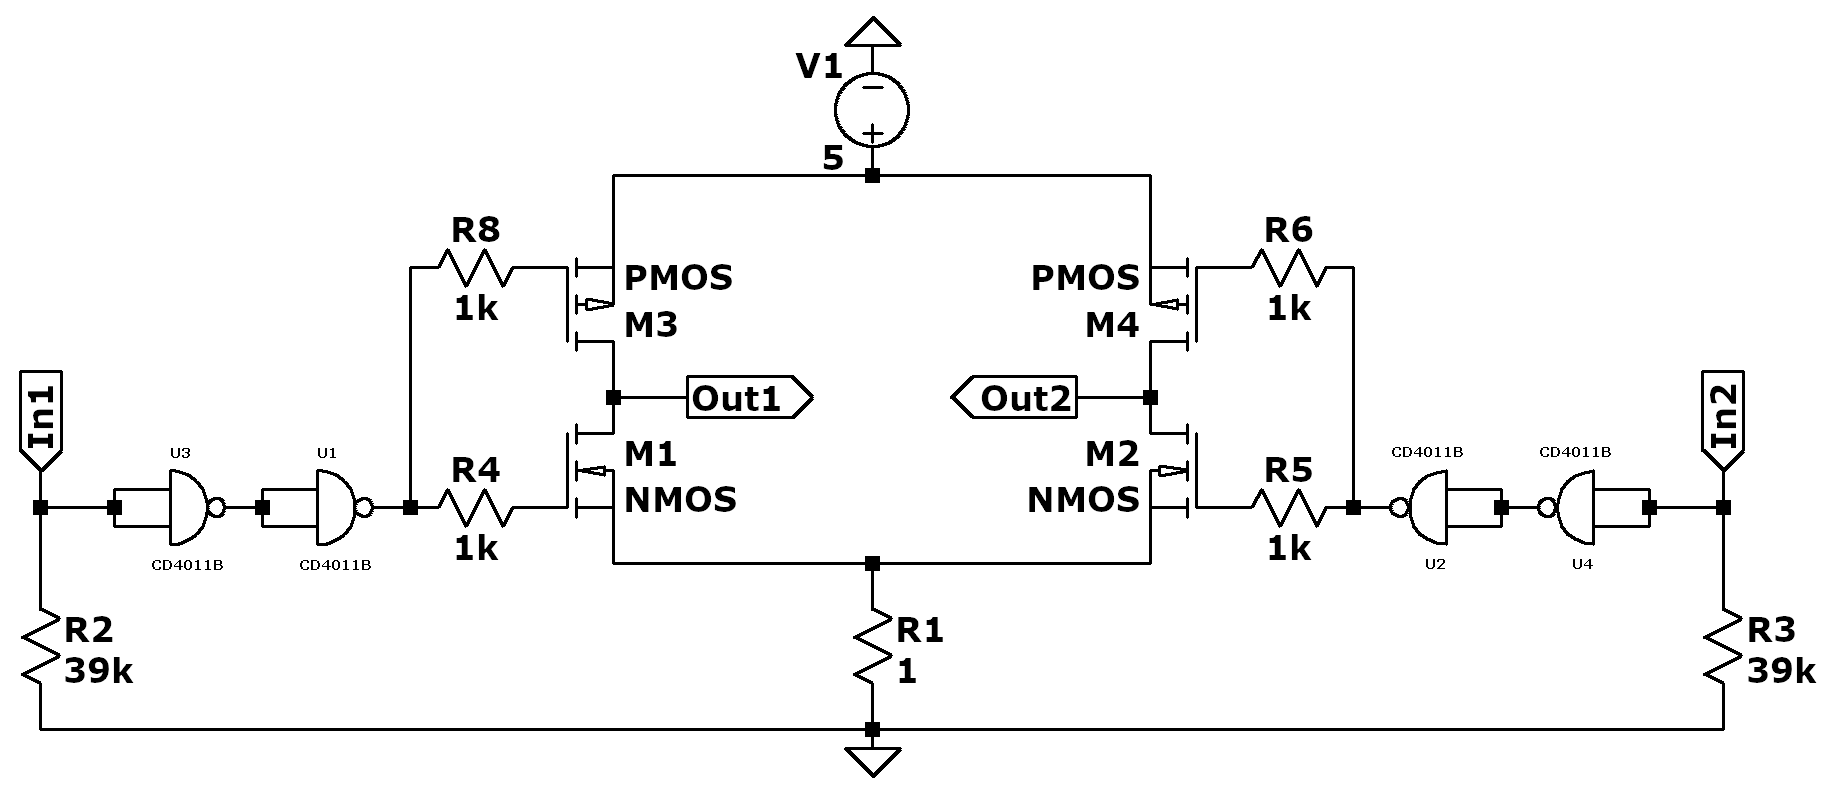
\includegraphics[width=\textwidth]{./images/circuit3.png}
	\end{columns}
		%\end{block}
	\end{frame}
	
	
	\section{Modellizzazione matematica}
	\subsection{Piattaforma di Gough-Stewart}
	\begin{frame}{Modellizzazione matematica}{Piattaforma di Gough-Stewart}

	\begin{columns}
	\column{0.4\textwidth}
	%Stabilizzazione di una pallina su un piano mediante l'uso di una piattaforma di Gough-Stewart.
	
	\begin{itemize}
		\item Descrizione vettoriale
		\item Problema attuatori rotativi
		\item Angoli per raggiungere una posizione nello spazio
	\end{itemize}
	\column{0.6\textwidth}
	\centering
\scalebox{0.5}{
\begin{tikzpicture}
 
\filldraw[fill=yellow!50,rotate around={-10:(0,7cm)},xshift=2cm,yshift=1cm] (0,7cm) ellipse (4cm and 2cm);
\filldraw [fill=red!50](0,0) ellipse (5cm and 2.5cm);
\draw [-latex, thick] (0,0) -- node[anchor=south]{$\hat b_i$}(5cm,0);
\draw [-latex, thick] (0,0) -- node[anchor=east]{$\hat T$}(2.15cm,7.65cm);
\draw [-latex, thick] (0,0) -- node[anchor=north]{$\hat q_i$}(6.1cm,6.95cm);
\draw [-latex, thick] (5cm,0) -- node[anchor=west]{$\hat l_i$}(6.1cm,6.95cm);
\draw[-latex, thick,rotate around={-10:(0,7cm)},xshift=2cm,yshift=1cm] (0cm,7cm) -- node[anchor=south]{$\hat p_i$}(4cm,7cm);
\filldraw [fill=black] (0,0) circle (2pt) node[yshift= -0.25cm] {$O$} node[xshift= -2cm] {Base};
\filldraw [fill=black] (5cm,0) circle (2pt) node[anchor=west]{$B_i$};
\filldraw [fill=black] (2.15cm,7.65cm) circle (2pt) node[yshift= 0.25cm] {$O'$} node[xshift= -2cm] {Piattaforma};
\filldraw [fill=black] (6.1cm,6.95cm) circle (2pt) node[anchor=west]{$P_i$};
\draw [-latex, thick] (-1,-1.5) -- node[anchor=north]{$\hat i$}(0cm,-1.5cm);
\draw [-latex, thick] (-1,-1.5) -- node[anchor=east]{$\hat k$}(-1cm,-0.5cm);
\draw [-latex, thick,rotate around={-120:(-1,-1.5cm)}] (-1,-1.5) -- node[anchor=east]{$\hat j$}(-0.5cm,-1.5cm);

\draw [-latex, thick,rotate around={-10:(0,8.5cm)}] (0,8.5) -- node[anchor=north]{$\hat {i'}$}(1cm,8.5cm);
\draw [-latex, thick,rotate around={-10:(0,8.5cm)}] (0,8.5) -- node[anchor=east]{$\hat {k'}$}(0cm,9.5cm);
\draw [-latex, thick,rotate around={-130:(0,8.5cm)}] (0,8.5) -- node[anchor=east]{$\hat {j'}$}(0.5cm,8.5cm);

\end{tikzpicture}
}
	\end{columns}
		%\end{block}
	\end{frame}
	
	
	
	\subsection{Controllore PID}
	\begin{frame}{Modellizzazione matematica}{Controllore PID}

	\begin{itemize}
		\item PID teorico
		\item Miglioramenti pratici impiegati
		\item Taratura euristica
	\end{itemize}
	\vspace{0.5cm}
	\centering
\scalebox{0.6}{
\begin{tikzpicture}[font=\small,thick]
 
% Start block
\node[draw,
    circle,
    minimum width=1cm,
     text centered] (block1) {$\Sigma$};
    
    % Power and voltage variation
\node[draw,
    right=of block1,
    minimum width=1cm,
    minimum height=1cm, xshift= 1cm
] (block2) {$K_i$};

\node[draw,
    right=of block2,
    minimum width=1cm,
    minimum height=1cm,
     text centered
] (int) {$\Sigma_{t_k}$};

\node[draw, right=of int,
    minimum width=1cm,
    minimum height=1cm,
     text centered
] (filter4) {$\Lambda$};


\node[draw, right=of int, 
    circle,
    minimum width=1cm, xshift=2cm,
     text centered] (S) {$\Sigma$};
    
\node[draw, right=of S,
    minimum width=1cm,
    minimum height=1cm,
     text centered
] (filter3) {$\Lambda$};

\node[draw,
    right=of filter3,
    minimum width=2cm,
    minimum height=1cm,
    text width=2cm, text centered
] (block3) {Piattaforma Stewart};

\node[draw,
    right=of block3,
    minimum width=2cm,
    minimum height=1cm,
    text width=2cm, text centered
] (block4) {Piano resistivo};
 
\node[draw,
    above=of block2,
    minimum width=1cm,
    minimum height=1cm,yshift=-0.5cm
] (P) {$K_p$};

\node[draw,
    below=of block2,
    minimum width=1cm,
    minimum height=1cm,yshift=0.5cm
] (D) {$K_d$};

\node[draw,
    right=of D,
    minimum width=1cm,
    minimum height=1cm,
     text centered
] (der) {$\Delta_{t_k}$};

\node[draw,
    right=of der,
    minimum width=1cm,
    minimum height=1cm,
     text centered
] (filter1) {$\Phi$};

\node[draw,
    minimum width=1cm,
    minimum height=1cm,
     text centered, xshift=19cm, yshift=-1.5cm
] (filter2) {$\Phi$};



% Arrows
\draw [-latex] (-2cm,0cm) -- node[anchor=south]{$x[k]$}(block1)node[xshift=-0.75cm,yshift=-0.25cm]{$+$}node[xshift=0.25cm,yshift=-0.75cm]{$-$};
\draw [-latex] (block1) edge (block2)node[anchor=south, xshift=1cm]{$e[k]$};
\draw [-latex](1.5,-3) |- (D);
\draw [-latex](1.5,0) |- (P);
\draw [-latex](D) edge (der);
\draw [-latex](block2) edge (int);
\draw [-latex](D) edge (der);
%\draw [-latex](int) -- (S)node[anchor=south, xshift= 1cm]{$c[k]$};
\draw [-latex](P) -| (S)node[xshift=0.25cm,yshift=0.75cm]{$+$}node[xshift=-0.75cm,yshift=0.25cm]{$+$}node[xshift=-0.25cm,yshift=-0.75cm]{$+$};
\draw [-latex]	(filter1) -| (S);
\draw [-latex]	(filter4) -- (S);
\draw [-latex]	(int) -- (filter4);
\draw [-latex]	(der) -- (filter1);
\draw [-latex]	(S) edge (filter3);	
\draw [-latex]	(filter3) edge (block3);	
\draw [-latex]	(block3) edge (block4);
\draw [-latex]	(block4) -- (20,0);	
\draw 	(19,0)node[anchor=south]{$u[k]$} -- (filter2);
\draw (filter2) -- (19,-3);		  
\draw [-latex]	(19,-3) -| (block1);	
\end{tikzpicture}
}
		%\end{block}
	\end{frame}	
	
	
	
	\subsection{Piano inclinato}
	\begin{frame}{Modellizzazione matematica}{Piano inclinato}

	\begin{itemize}
		\item Modello fisico
		\item Funzione di trasferimento piano inclinato
		\item Analisi di stabilità impiegando controllore PID
	\end{itemize}
	\centering
\scalebox{1}{
\begin{tikzpicture}[font=\small,thick]
%\draw [-latex](-3,0) -- (3,0cm)node[anchor=south]{$x$};
\filldraw [fill=black!30, rotate around={7:(0,0cm)}](0cm,0cm) rectangle (10,-0.1cm);%node[xshift=-1cm]{$\beta=\frac{\pi}{2}$};
\filldraw [fill=white, rotate around={7:(0,0cm)}](8,0.5) circle (0.5cm);
\draw [-latex, red, rotate around={7:(0,0cm)}](8,0.5) -- (6,0.5cm)node[anchor=south]{$sin(\theta)\cdot m\cdot g$};
\draw [-latex, red, rotate around={7:(0,0cm)}](8,0) -- (9,0cm)node[anchor=south]{$F_a$};
\draw [-latex, rotate around={7:(0,0cm)}](8.5,1.5) -- node[anchor=south]{$a$}(7.5,1.5cm);
%\draw [ rotate around={7:(0,0cm)}](8,0) -- node[anchor=west,yshift=0.1cm, rotate around={7:(0,0cm)}]{$r$}(8,0.5cm);
\draw [-latex, rotate around={0:(0,0cm)}](7.88,1.5) -- (7.88,0.2cm)node[anchor=west]{$m\cdot g$};
\draw [ -latex, rotate around={7:(0,0cm)}](8.7,0.7cm)node[anchor=west,xshift=-0.3cm,yshift=0.5cm]{$\omega$} arc (10:90:0.7cm);
%\draw [ rotate around={7:(0,-0.1cm)}](0,-0.1cm)node[anchor=west,xshift=-0.3cm,yshift=0.5cm]{$\omega$} arc (10:90:0.7cm);
\draw [rotate around={0:(0,0cm), xshift=0mm}](0mm,-0.1cm)node[xshift= 1.75cm,yshift= 0cm]{$\theta$} -- (15mm,-0.1cm) arc  (0:7:15mm)-- cycle;

\filldraw [fill=black, rotate around={7:(0,0cm)}] (8,0.5) circle (1pt);
\filldraw [fill=black, rotate around={7:(0,0cm)}] (8+0.3535,0.5+0.3535) circle (1pt);
\draw [rotate around={7:(0,0cm)}] (8,0.5) -- node[anchor=east, yshift=0.1cm, xshift=0.1cm]{$r$}(8+0.3535,0.5+0.3535);
\filldraw [fill=black, rotate around={7:(0,0cm)}] (8,0) circle (1pt);
\end{tikzpicture}
}
		%\end{block}
	\end{frame}
	
	\section{Realizzazione pratica}
	\subsection{Assemblaggio}
	\begin{frame}{Realizzazione Pratica}{Assemblaggio}

	\begin{columns}
	\column{0.3\textwidth}
	%Stabilizzazione di una pallina su un piano mediante l'uso di una piattaforma di Gough-Stewart.
	
	\begin{itemize}
		\item Modello e stampa 3D
		\item Servomotori
		\item Piano resistivo
		\item Ponte ad H
	\end{itemize}
	\column{0.7\textwidth}
	\centering 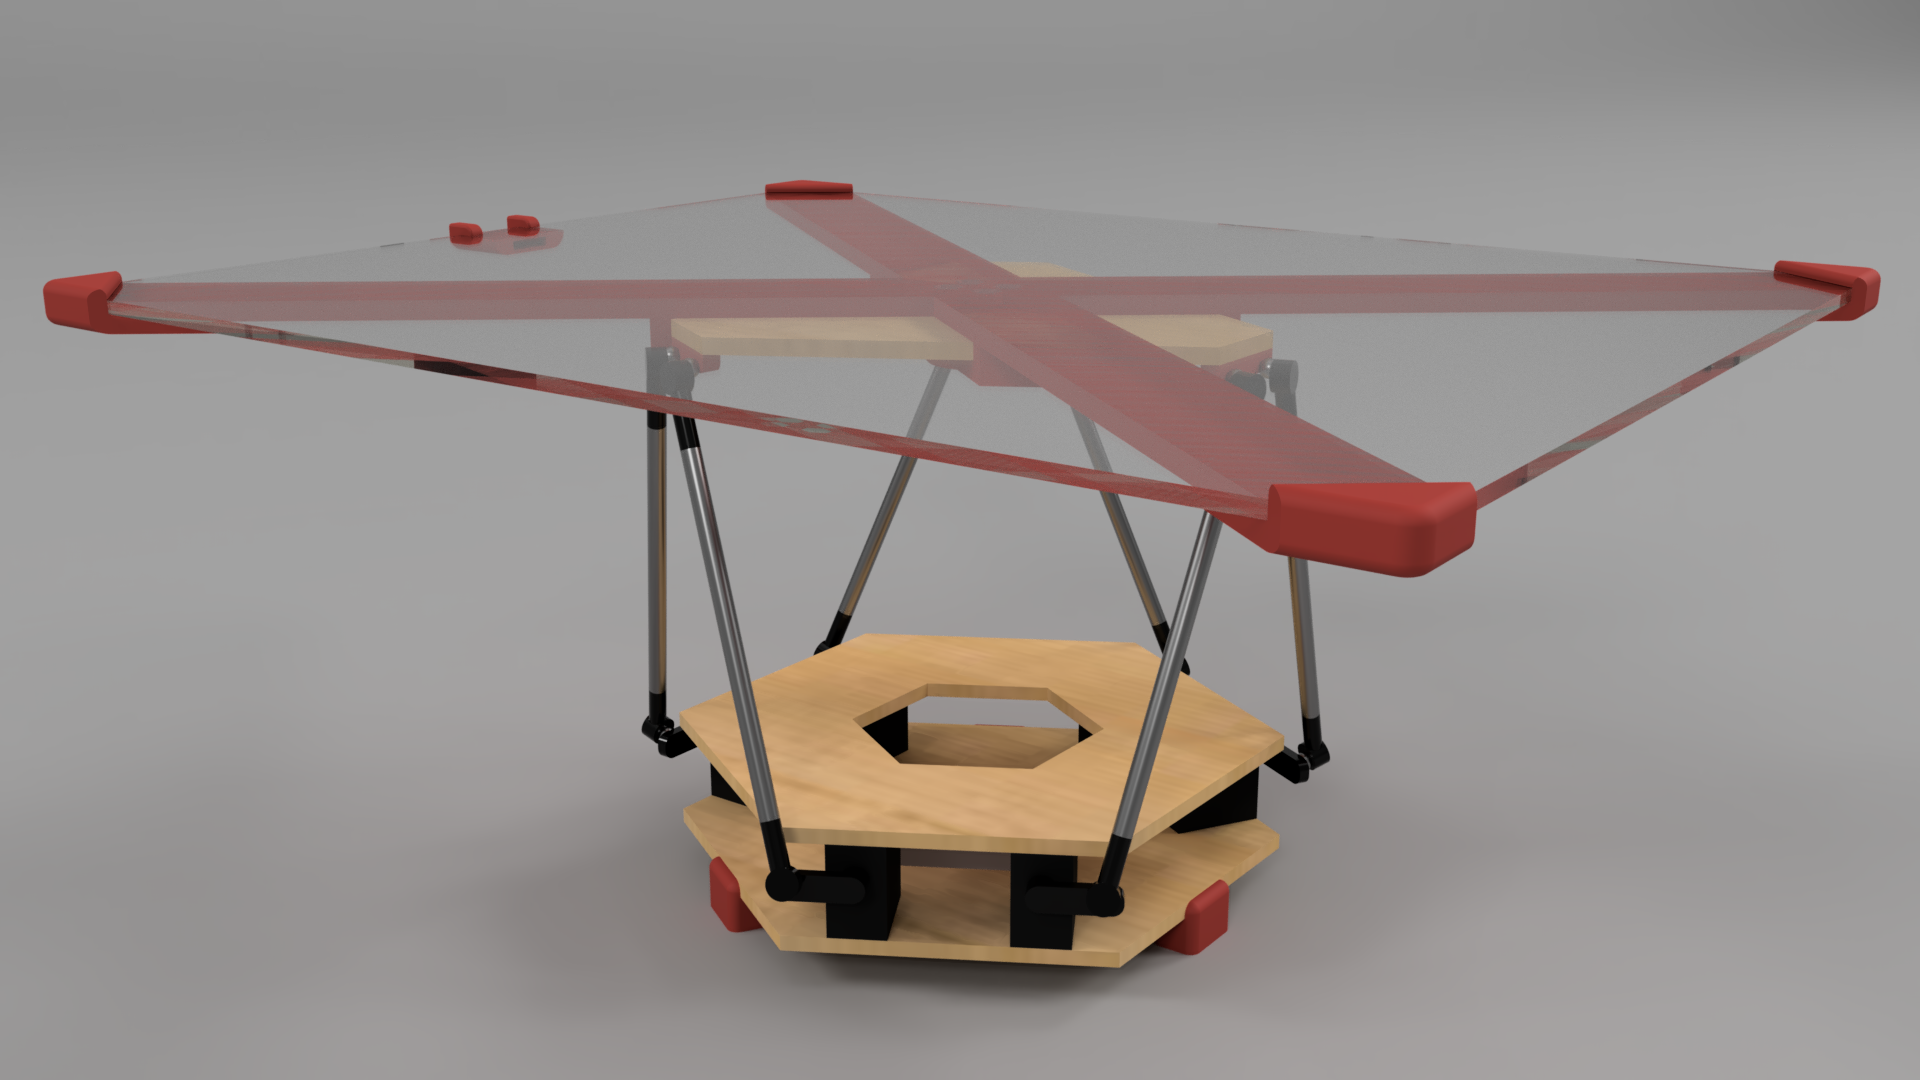
\includegraphics[width=\textwidth]{./images/stewart.png}
	\end{columns}
		%\end{block}
	\end{frame}
	
	\subsection{Programmazione}
	\begin{frame}{Realizzazione Pratica}{Programmazione}
	\begin{columns}
	\column{0.5\textwidth}
	\begin{itemize}
	
		\item Controllo semplice e intuitivo:\\ 
		\small \texttt{setPosition(x, y, z, rol, pit, yaw);}
		\item Controllo raggiungibilità posizione
		%\item Implementazione controllore PID: 	\\\texttt{setPosition(0,0,108,radians(tiltX),radians(tiltY),radians(0));}
		
		\item Filtraggio dati con media e filtro passa basso
		\item Analisi della temporizzazione all'oscilloscopio
		\item Programmazione figure di Lissajous
	\end{itemize}
	\column{0.5\textwidth}
	\centering 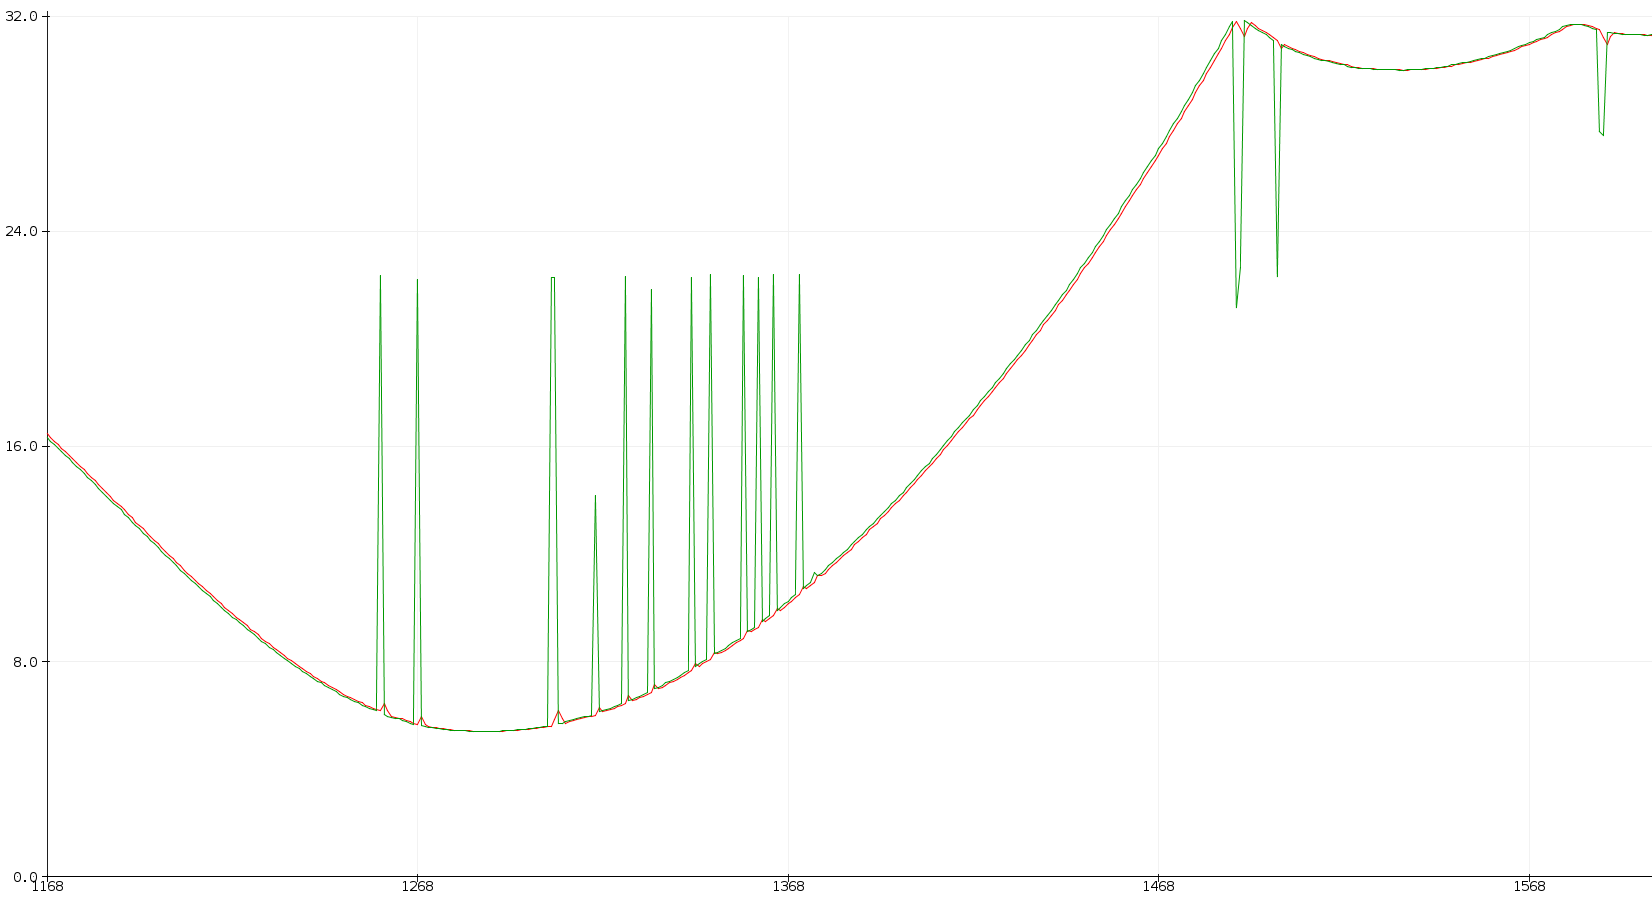
\includegraphics[width=0.65\textwidth]{./images/filtraggio2.png}\\
	\vspace{0.3cm}
	\centering 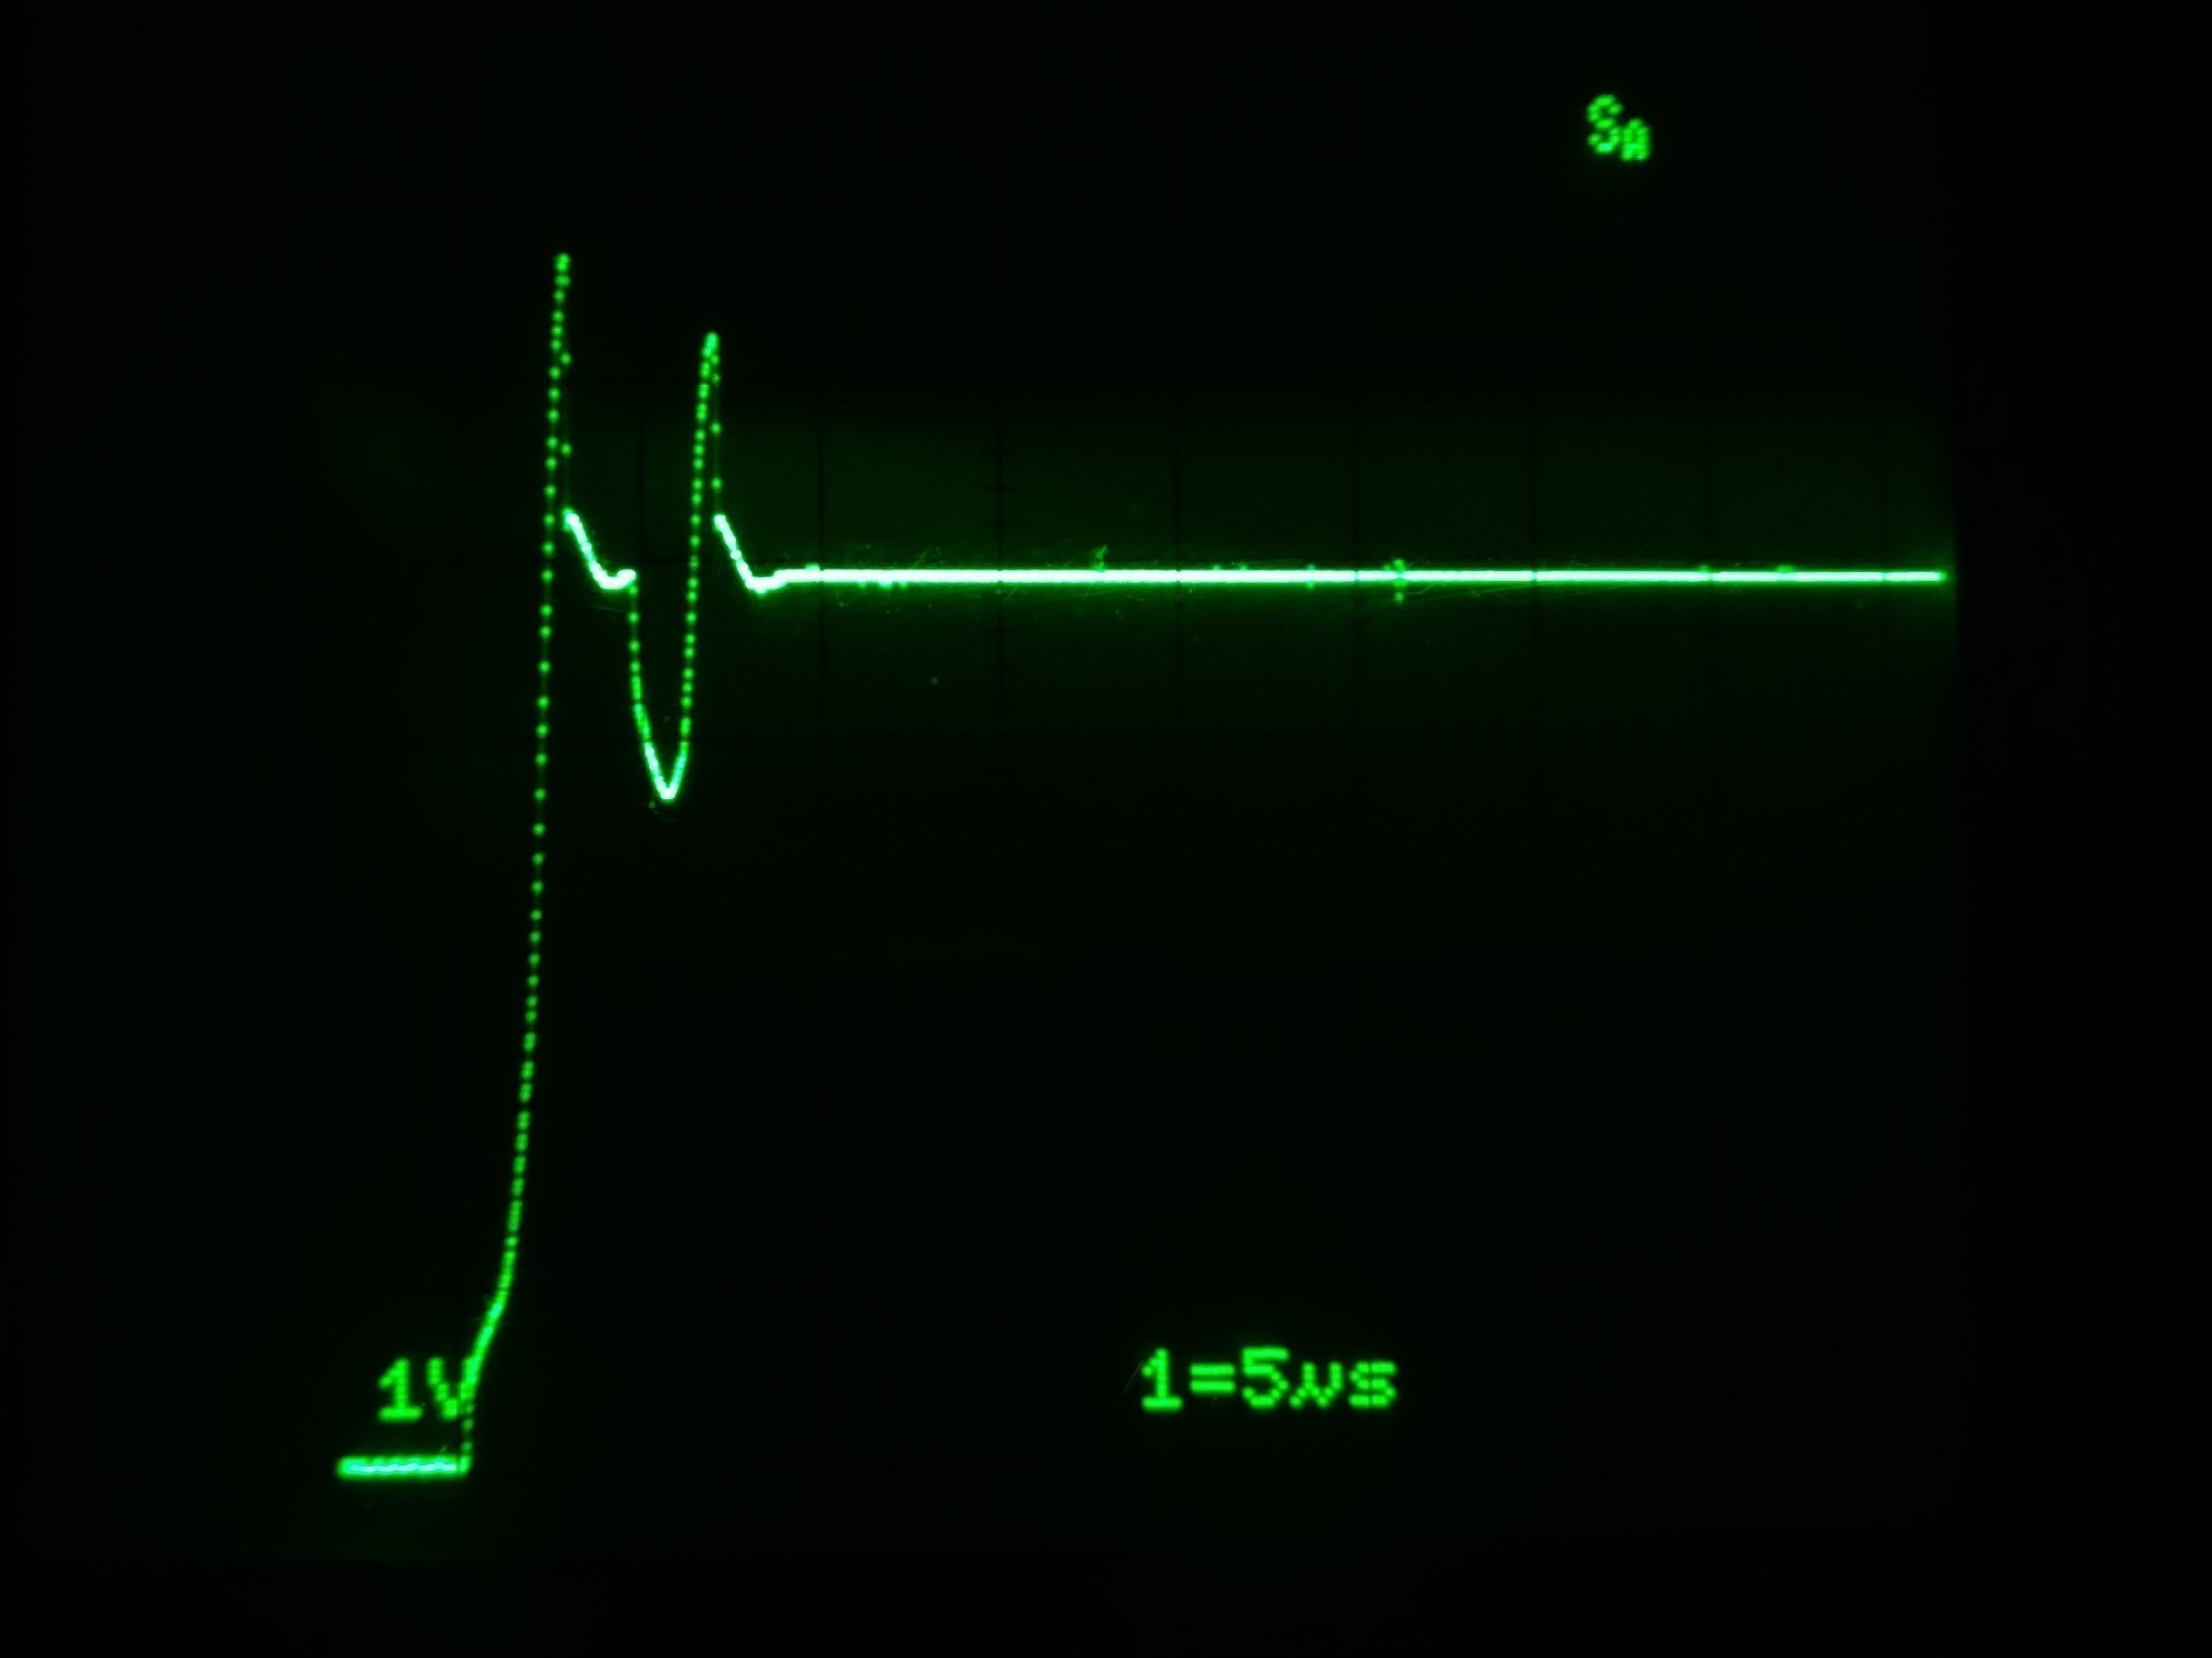
\includegraphics[width=0.65\textwidth]{./images/osc2.jpg}
	\end{columns}
	\end{frame}
	
	\section{Risultati}
	
	\subsection{Dimostrazione 6 gradi di libertà}
	\begin{frame}{Risultati}{Dimostrazione 6 gradi di libertà}
	\centering\movie[width=12cm, height=6.75cm, poster, autostart, repeat]{}{./images/test.mp4}
	\end{frame}
	\subsection{Dimostrazione stabilizzazione}
	\begin{frame}{Risultati}{Dimostrazione stabilizzazione}
	\centering\movie[width=12cm, height=6.75cm, poster, autostart, repeat]{}{./images/test.mp4}

	\end{frame}
	
	\subsection{Dimostrazione setpoint dinamico}
	\begin{frame}{Risultati}{Dimostrazione setpoint dinamico}
	\centering\movie[width=12cm, height=6.75cm, poster, autostart, repeat]{}{./images/test.mp4}

	\end{frame}
	
	\begin{frame}[plain,noframenumbering]
	\standoutpage{\bfseries\huge Grazie per l'attenzione!}
	\end{frame}

\end{document}
		